\subsection{Domänenmodellierung}
\label{sec:Kap-6.3.2}

Ein Domänenmodell besteht aus statischen und dynamischen Sichten auf die Domäne. In Lektion~2 % todo Lektion~\ref{sec:Lektion-2}
haben Sie mit dem Domänenklassendiagramm eine statische Sicht auf die Domäne gesehen: Objekte bzw. Klassen, ihre Eigenschaften und Beziehungen zueinander. Im letzten Abschnitt haben Sie mit dem Anwendungsfalldiagramm Möglichkeiten kennengelernt, dynamische Aspekte der Domäne zu modellieren: Tätig\-keiten von Akteuren in der Domäne. Bisher nur ab und an kurz erwähnt, haben wir einen weiteren wichtigen Bestandteil der Domänenmodellierung, die Erstellung eines Glossars.

\vspace{2mm} %%% für Druck

\minisec{Glossar}

Ein Glossar beinhaltet Erläuterungen für das Vokabular der Domäne, das im Rahmen der Entwicklung des Softwareprodukts erläuterungsbedürftig ist. Welches 
\linebreak %%% für Druck
Vokabular der Domäne ist erläuterungsbedürftig und welches nicht? Gehören im Zoobeispiel die Tierarten ins Glossar? Bei Schaf und Ziege würden die meisten von Ihnen vermutlich nein sagen, bei Gelbzahnmeerschweinchen die meisten jedoch ja. 

\vspace{2mm} %%% für Druck

Letztendlich gibt es keine Antwort, welcher Begriff erläuterungsbedürftig ist und welcher nicht. In jedem Fall gehören alle die Objekte, Akteure, Konzepte, Tätigkeiten, Prozessverben, Zusammenhänge etc. ins Glossar, die irgendwann im Laufe des Requirements Engineering in Diskussionen mal zu Verständnisproblemen geführt haben. Das Glossar wächst also kontinuierlich an und ist im Übrigen auch nicht am Ende des Requirements Engineering zwingend abgeschlossen. In manchen Projekten werden grundsätzlich alle in Modellen und Anforderungen vorkommenden Begriffe der Domäne ins Glossar aufgenommen, dann eben auch Schaf und Ziege.

\vspace{2mm} %%% für Druck

Zu jedem Eintrag im Glossar sollten mindestens folgende Informationen enthalten sein:
\begin{itemize}
	\item der Begriff
	\item der Typ des Begriffs, z.B. ein Akteur (Nagetierpfleger) oder eine Aktion in einem Geschäftsprozess (Bonuspunkte einsetzen)
	\item die Erläuterung des Begriffs
	\item Verweise auf inhaltlich verwandte Begriffe bzw. Konzepte. Zum Beispiel beim Gelbzahnmeerschweinchen der Verweis auf den Glossareintrag des Zwergmeerschweinchens 
	\item Welche synonymen Begriffe gibt es: Synonyme sind unterschiedliche Begriffe für denselben Sachverhalt. Die Verwendung von Synonymen sollte man idealerweise ganz vermeiden. Man wird sie aber in Dokumenten und Grafiken finden, die die Stakeholder liefern. Insofern ist es wichtig, sie im Glossar aufzuführen.
	\item Handelt es sich bei diesem Begriff um ein Homonym? Ein Begriff ist ein \mbox{Homonym}, wenn er mehrere abweichende Bedeutungen hat, wie zum Beispiel die Bank, bei der ich mein Konto habe und die Bank, auf der ich im Park sitzen kann. Sofern Homonyme im Vokabular der Domäne vorkommen, empfiehlt es sich, für eine der Bedeutungen einen abweichenden Begriff zu verwenden, zum Beispiel Geldinstitut für den ersten Bank-Begriff.
	\item Ggf. Referenzen auf die Requirements Engineering-Dokumente, in denen der Begriff verwendet wird. Das ist allerdings sehr aufwändig durchzuhalten, da man das Glossar bei jedem neuen Diagramm etc. an mehreren Stellen ergänzen müsste.
\end{itemize}

\pagebreak %%% für Druck

\minisec{Die Bedeutung der Domänenmodellierung}

Das wichtigste Ziel der Domänenmodellierung ist das explizit Machen von implizitem Wissen. Betrachten Sie die folgende Aussage.

\sttpAnforderungText{Man kann Führungen durch den Zoo online buchen. Die Teilnahme an Fütterungsführungen ist aber nur für Gruppen bis 5 Personen möglich.}

\vspace{\baselineskip} %%% für Druck

Sind Führungen und Fütterungsführungen unterschiedliche Dinge? Einem Zoo-
\linebreak %%% für Druck
Domänenexperten wird das klar sein und er wird vielleicht nicht explizit darauf hinweisen. Modelliert man die Beziehung zwischen Zoobesuchern und Führungen aber in einem Domänenklassendiagramm, wird der Domänenexperte darauf hinweisen, dass die in Abbildung~\ref{fig:zoofuehrung} oben %%% links 
gezeigte Modellierung falsch ist, wenn eine Struktur wie in der unteren %%% rechten 
Hälfte der Abbildung zutrifft.

\vspace{\baselineskip} %%% für Druck
\vspace{2mm} %%% für Druck

\begin{figure}[h!]
	\centering
	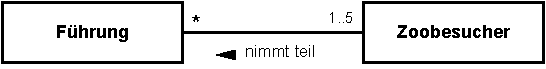
\includegraphics{Bilder/Kapitel-6/zoofuehrung_links.pdf}
	\vspace{\baselineskip}
	{\color{FernUni-MI-green}\rule{120mm}{1pt}} % horizontale farbige Linie
	\vspace{\baselineskip}
	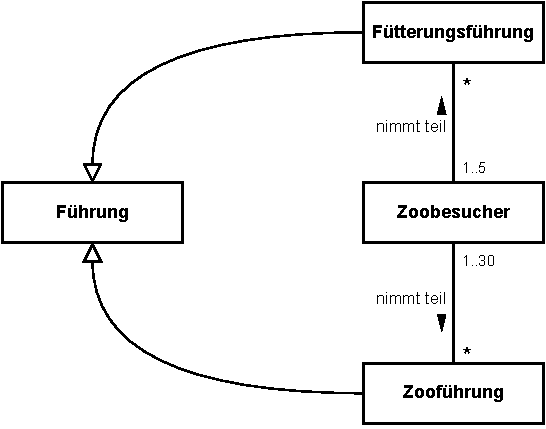
\includegraphics{Bilder/Kapitel-6/zoofuehrung_rechts.pdf}
	\caption{Zooführung}
	\label{fig:zoofuehrung}
\end{figure}

\vspace{\baselineskip} %%% für Druck

Wenn man im Requirements Engineering die Domänenmodellierung vernachlässigt, werden einem sehr sicher Anforderungen an das zu entwickelnde Softwareprodukt entgehen. Daher sollten Sie die Domäne wie einen Stakeholder behandeln und ihre „Bedürfnisse“ mit berücksichtigen. 